%----------------------------------------------------------------------------------------
%	PAQUETES
%----------------------------------------------------------------------------------------

\documentclass[12pt,spanish]{article} % Default font size is 12pt, it can be changed here


\usepackage[margin=1in]{geometry}


\geometry{a4paper} % Set the page size to be A4 as opposed to the default US Letter

\usepackage{graphicx} % Required for including pictures

\usepackage{float} % Allows putting an [H] in \begin{figure} to specify the exact location of the figure
\usepackage{wrapfig} % Allows in-line images such as the example fish picture

\usepackage{lipsum} % Used for inserting dummy 'Lorem ipsum' text into the template

\linespread{1.} % Line spacing

\setlength{\parskip}{0.3cm} % Paragraph vertical spacing

%\setlength\parindent{0pt} % Uncomment to remove all indentation from paragraphs

\graphicspath{{Pictures/}} % Specifies the directory where pictures are stored

% Specify Spanish packages
\usepackage[spanish]{babel}
\selectlanguage{spanish}
\usepackage[utf8]{inputenc}

% Table
\usepackage{tabularx}
\usepackage{array}

% Fonts con colores
\usepackage{xcolor}

\usepackage{caption}

% Para codigo en Python
\definecolor{mygreen}{rgb}{0,0.6,0}
\definecolor{mygray}{rgb}{0.5,0.5,0.5}
\definecolor{mymauve}{rgb}{0.58,0,0.82}
\definecolor{mygray}{rgb}{0.95, 0.95, 0.95}
\usepackage{listings}
\usepackage{color}
\lstset{ %
  backgroundcolor=\color{mygray},   % choose the background color
  basicstyle=\footnotesize\ttfamily,        % size and type of fonts used for the code
  breaklines=true,                 % automatic line breaking only at whitespace
  captionpos=b,                    % sets the caption-position to bottom
  commentstyle=\color{mygreen},    % comment style
  escapeinside={\%*}{*)},          % if you want to add LaTeX within your code
  keywordstyle=\color{blue},       % keyword style
  stringstyle=\color{mymauve},     % string literal style
  frame=single
}

\usepackage{algorithm,refcount}          %  float wrapper for algorithms.
\usepackage{algpseudocode}      % layout for algorithmicx
\usepackage{amsmath}            % AMS mathematical facilities for LATEX
\floatname{algorithm}{Algoritmo}

% Para floor y ceil
\usepackage{mathtools}
\DeclarePairedDelimiter\ceil{\lceil}{\rceil}
\DeclarePairedDelimiter\floor{\lfloor}{\rfloor}

% Para poder usar equation* y tener ecuaciones sin numero
\usepackage{amsmath,amssymb,amsthm}

\usepackage[final]{pdfpages}

\definecolor{violeta}{HTML}{400080}
\definecolor{azul}{HTML}{0033CC}
\definecolor{rojo}{HTML}{FF0000}

% Para headers y footers
\usepackage{fancyhdr}
 
\fancyhf{}
\rhead{Federico Rafael García García}
\lhead{Trabajo 3: Programación}
\cfoot{\thepage}

% Para referencias
\usepackage[backend=biber]{biblatex}
\addbibresource{references.bib}


\begin{document}

\abovedisplayshortskip=0pt
\belowdisplayshortskip=0.0cm
\abovedisplayskip=0.0cm
\belowdisplayskip=0pt


%----------------------------------------------------------------------------------------
%	TITLE PAGE
%----------------------------------------------------------------------------------------

\begin{titlepage}

\newcommand{\HRule}{\rule{\linewidth}{0.5mm}} % Defines a new command for the horizontal lines, change thickness here

\center % Center everything on the page

\LARGE Universidad de Granada\\[1cm] % Name of your university/college


\includegraphics[scale=.2]{logo}

\HRule \\[0.5cm]
{ \LARGE \bfseries Trabajo 3: Programación}\\[0.1cm] % Title of your document
\HRule \\[0.5cm]

\vspace{1.0cm}

\Large \textbf{Aprendizaje Automático}

\vspace{0.75cm}

\large Federico Rafael García García

\large Curso 2018/2019



{\today} % Date, change the \today to a set date if you want to be precise

%\includegraphics{Logo}\\[1cm] % Include a department/university logo - this will require the graphicx package

\vfill % Fill the rest of the page with whitespace

\end{titlepage}

%----------------------------------------------------------------------------------------
%	INDICE
%----------------------------------------------------------------------------------------

\tableofcontents % Include a table of contents

\newpage % Begins the essay on a new page instead of on the same page as the table of contents 

\pagestyle{fancy}

%----------------------------------------------------------------------------------------
%	EJERCICIO 1
%----------------------------------------------------------------------------------------

\section{Dígitos manuscritos}

\subsection{Particiones training y test}

La base de datos de dígitos manuscritos consta de dos ficheros de texto, uno para \textit{training} (optdigits.tra) y otro para \textit{test} (optdigits.tes), por lo que no hará falta particionar los datos al ya venir preparados. Los datos fueron obtenidos a través de los siguientes enlaces:

\noindent
{\small \texttt{https://archive.ics.uci.edu/ml/machine-learning-databases/optdigits/optdigits.tes}}

\noindent
{\small \texttt{https://archive.ics.uci.edu/ml/machine-learning-databases/optdigits/optdigits.tra}}

\subsection{Visualización y preprocesado de datos}

Cada línea de cada fichero consta de 65 valores enteros separados por comas. Los 64 primeros son las características, mientras que el último es la etiqueta: $0, 1, ..., 9$. Las 64 características representan una matriz 8x8 con valores en [0-16]: son imágenes de los dígitos manuscritos en escala de gris.

Con el fin de entender mejor los datos con los que se trabajará, se ha decidido seleccionar 10 elementos de cada dígito y visualizarlos. Para ello se ha transformado cada vector de 64 características en una matriz 8x8, y cada uno se ha copiado a una región de una matriz 80x80. En la figura \ref{fig:digitos} se pueden ver 100 dígitos manuscritos.

\begin{figure}[H]
  \begin{center}
  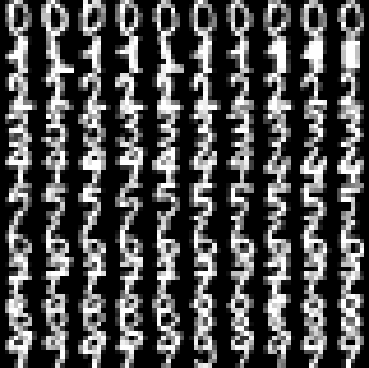
\includegraphics[scale=0.8]{digitos}
  \caption{Representación gráfica de 100 dígitos.}
  \label{fig:digitos}
  \end{center}
\end{figure}

Dado que el espacio es de 64 dimensiones, se ha decidido buscar alguna transformación que permita reducirlo, con las ventajas que ello significa: entrenamiento más rápido, mejor representación de los datos y un modelo más simplificado y claro de entender. Al poder ser los datos representados como imágenes, se ha decidido utilizar una transformación que utilice las siguientes características:

\begin{itemize}
\item \textit{Simetría vertical}: Se divide la matriz en dos mitades de 8x4, se restan, se obtiene el absoluto y se suman todos su valores. Cuanto menor sea el resultado, mayor es la simetría.
\item \textit{Intensidad superior}: Se divide la matriz en la primera mitad de 4x8 y se suman todos los valores.
\item \textit{Intensidad inferior}: Se divide la matriz en la segunda mitad de 4x8 y se suman todos los valores.
\end{itemize}

Se han elegido estas características ya que pueden diferenciar números simétricos (0, 1, 8, ...) de aquellos que no lo son (2, 3, 4 , ...) y en el caso de que haya el mismo nivel de simetría vertical, diferenciarlos según qué número tiene más intensidad en la parte superior o inferior (como en el caso del 6 y el 9). Se ha realizado por tanto la siguiente transformación de dimensión: $\mathbb{Z}^{64} \rightarrow \mathbb{Z}^3$.

Usando la función \texttt{Plot3D}, se pueden representar puntos 3D con diferente color según su etiqueta. En la figura \ref{fig:nube3d} se pueden ver los datos desde diferentes perspectivas.

\begin{figure}[H]
  \begin{center}
  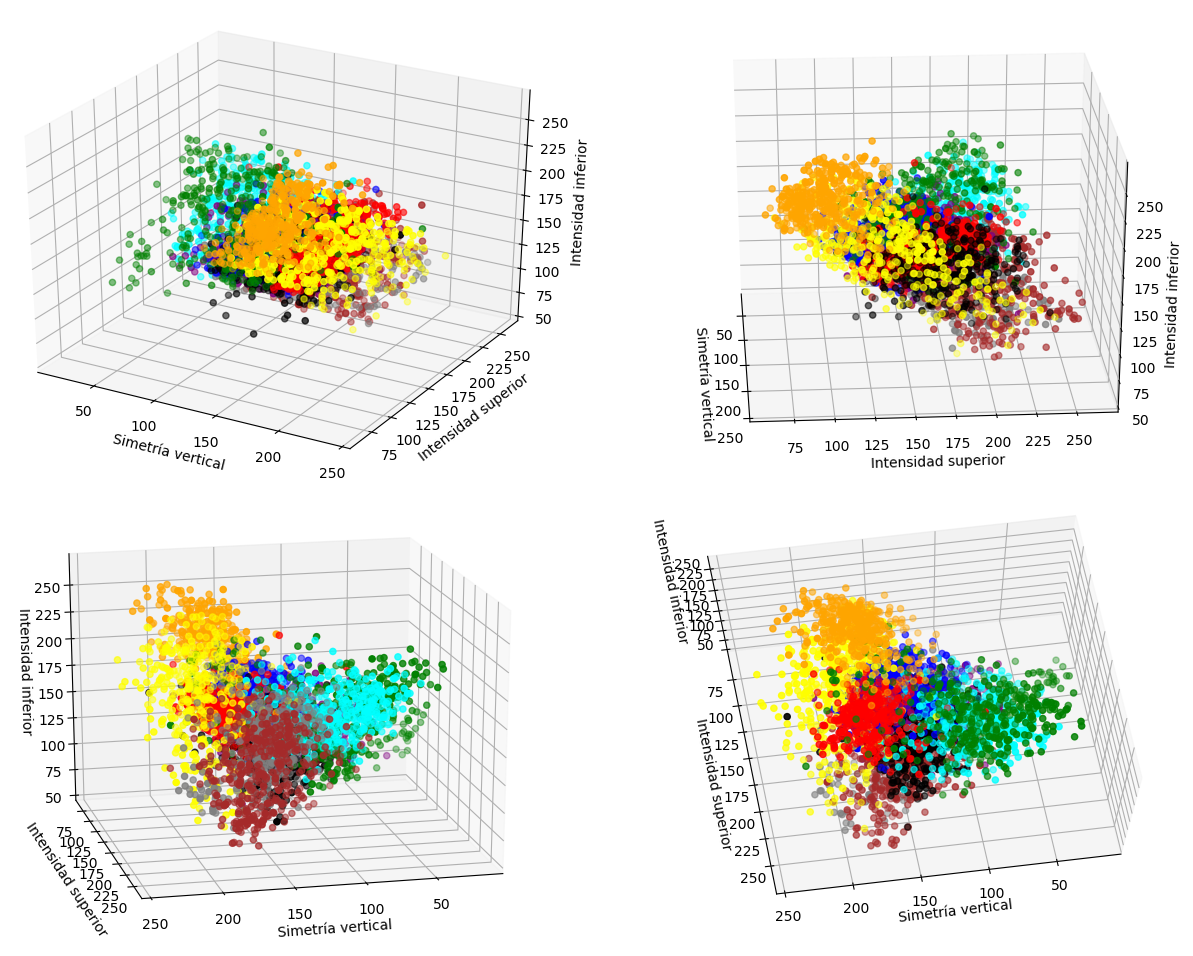
\includegraphics[scale=.5]{nube3d}
  \caption{Plot 3D de la transformación a simetría, intensidad superior e inferior.}
  \label{fig:nube3d}
  \end{center}
\end{figure}

Se aprecian diferentes \textit{clusters}, pero algunos no están bien diferenciados del resto.

Para comprobar que la transformación es de calidad y no se ha reducido la caracterización de los dígitos que permite diferenciarlos, se ha utilizado el algoritmo \textit{Knn Leave One Out} con $k=1$. En este algoritmo de clasificación, dado un elemento del conjunto se compara con el resto, buscando el elemento más similar, dado que probablemente su etiqueta sea igual al del más parecido. Una vez se ha encontrado, se comparan sus etiquetas; si son iguales, se tiene un acierto, y en caso contrario un fallo. El número de aciertos indicará si se es posible identificar un dígito del resto. No utilizamos el conjunto de test, con el fin de evitar influenciar el entrenamiento de alguna manera (\textit{bias}), razón por la cual usamos la técnica \textit{Leave One Out} para poder usar el propio conjunto de entrenamiento. Para acelerar los cálculos, se ha escogido el 10\% (en proporción para cada etiqueta) de los datos para ser comparado con todos los datos.

Para la comparación de un dígito con otro, se resta una a una las características de uno con el otro, se obtiene sus valores absolutos y finalmente se suman; cuanto menor sea este valor, existe mayor probabilidad de que los elementos tengan la misma etiqueta.

La ejecución de \textit{Knn} con el conjunto sin transformar, $\mathbb{Z}^{64}$,  ha resultado en un 97.08\% de aciertos; con el conjunto transformado a $\mathbb{Z}^3$ se ha obtenido una tasa de acierto del 42.18\%. Claramente, la transformación es pésima y no debería ser usada.

Se ha decidido utilizar otra transformación, de dimensión 16: cada característica es la suma de todos los valores de una fila o de una columna. De esta manera, se está comprimiendo toda la intensidad en una única fila o en una única columna. La ejecución de \textit{Knn} con este nuevo conjunto transformado en $\mathbb{Z}^{16}$ ha resultado en un 95.23\% de aciertos, un 1.85\% menos que los datos sin transformar. A cambio de un pequeño incremento del error, se ha reducido considerablemente la complejidad del problema.

Los datos pueden ser visualizados con dos histogramas. En la figura \ref{fig:histogramas} se puede ver la media de las características para todos los elementos de cada dígito: en azul se ve la suma de intensidad por fila y en rojo por columna. Por ejemplo, en el caso del dígito 1, puesto que se trata de un trazo vertical, la suma de intensidad de cada fila será similar; por ello las barras en azul tienen alturas similares. Al ser un único trazo vertical, las columnas centrales tendrán la mayor suma de intensidad, como se puede ver reflejado en las barras rojas.

\begin{figure}[H]
  \begin{center}
  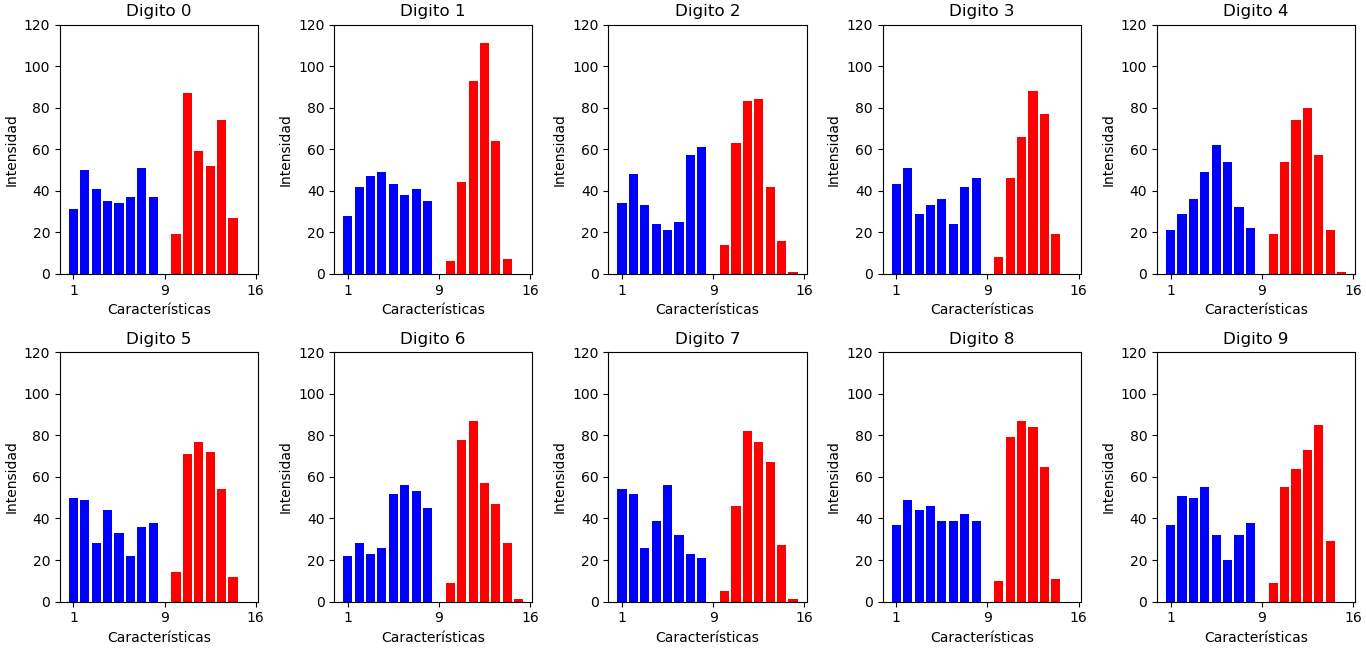
\includegraphics[scale=.46]{histogramas}
  \caption{Media de características en $\mathbb{Z}^{16}$ de todos los elementos de cada dígito. Las barras en azul representan las primeras 8 características, la suma de intensidades de cada fila. Las barras en rojo representan las últimas 8 características, la suma de intensidades de cada columna.}
  \label{fig:histogramas}
  \end{center}
\end{figure}

No se normalizaron las características, puesto que todas ellas tienen el mismo rango de valores.

Finalmente, se ha decidido reducir la dimensionalidad todavía más mediante eliminación, quitando características que no reduzcan la tasa de aciertos de \textit{Knn}; se pretende eliminar las características que no sean ``importantes''. En nuestro caso, serían las casillas de la fila o columna suma de intensidad que siempre tienen los mismos valores para todos los dígitos.

Para determinar las características importantes de las que no, se ha utilizado la \textit{varianza de la media de cada característica de todos los dígitos}. El proceso es el siguiente:

\begin{enumerate}
\item Para cada conjunto transformado de cada dígito, hacer la media de cada característica. Por ejemplo, para el conjunto de todos los elementos etiquetados como 0, obtener la media de la primera característica, de la segunda, etc.
\item Hacer la varianza de todas las medias de una característica. Por ejemplo, dada la media de la primera característica del conjunto 0, y el conjunto 1, etc. obtener la varianza.
\end{enumerate}

Cada varianza nos permite saber qué tan diferente son las medias de una característica. Si la varianza de una característica es baja, significa que todos los dígitos tienen valores casi iguales para esa característica. Esto significa que no ayuda a distinguir un dígito de otro. Estas características pueden ser eliminadas.

Dado que no existe una clara definición de lo que es una \textit{varianza baja}, esta se ha hallado mediante experimentación. Se ha determinado que eliminar características con varianza menor a 10 no afecta la tasa de aciertos de \textit{Knn}. De esta manera, se ha conseguido reducir la dimensión de 16 a 14. Se eliminaron las características 9 y 16: la primera y última característica del histograma de columnas. Se puede ver en el gráfico que los valores de las características 9 y 16 son cero o extremadamente bajos.

\subsection{Funciones a usar}

Al tener clústers claramente diferenciables (según los resultados obtenidos con \textit{KNN-LOU}), se utilizarán funciones lineales para clasificar los dígitos: se obtendrán hiperplanos que permitan separar clústers entre sí. Para ello se utilizará un clasificador de Regresión Logística Multinomial. Usamos Regresión Logística para obtener la probabilidad de que un elemento pertenezca a una clase u otra, es decir, que sea un dígito u otro, y Multinomial al haber múltiples clases. Cada elemento será clasificado con la clase que tenga mayor probabilidad.

En el clasificador se utilizará el algoritmo de \textit{newton-cg}, basado en el ``Método de Newton''.

No se ha utilizado regularización, por lo que el parámetro \texttt{C}, que define la inversa de la fuerza de regularización, se ha dejado en su valor por defecto de 1. Se ha decidido así puesto que se asume una gran variabilidad en los manuscritos digitalizados: la forma de escritura es muy personal, y será muy diferente de un individuo a otro. Por ello asumimos que no ocurrirá \textit{overfitting}.

\subsection{Entrenamiento y test}

Se ha entrenado ejecutando las funciones de \textit{SK Learn} con el conjunto de entrenamiento transformado y reducido (\textit{xf\_train}) y el conjunto de etiquetas (\textit{y\_train}):

\begin{center}
\texttt{softReg = LogisticRegression(multi\_class='multinomial', solver='newton-cg', max\_iter=200)}

\texttt{softReg.fit(xf\_train, y\_train)}
\end{center}

Se ha entrenado con 200 iteraciones, puesto que con una cantidad mayor no se han obtenido mejor resultados (no se ha reducido $E_{in}$).

Luego se ha transformado y reducido el conjunto de test y se han obtenido las predicciones: un array con la clase predecida de cada elemento del conjunto de test \textit{xf\_test}:

\begin{center}
\texttt{predicciones = softReg.predict(xf\_test)}
\end{center}

Al tener predicciones de etiquetas que se pueden clasificar como ``correcta'' o ``incorrecta'', el error es MAE; en un bucle se ha comparado cada clase predecida con la etiqueta del elemento. Con ello se ha obtenido el error; la tasa de acierto es por tanto $(1-E) \times 100$.

En el caso de $E_{out}$, este ha sido 0.09961 (tasa de acierto de casi 90.04\%).

En el caso de $E_{in}$, este ha sido 0.08553 (tasa de acierto de casi 91.45\%).

\subsection{Conclusiones}

Se puede ver el gran efecto que puede tener el preprocesado en la clasificación: se ha de ser cuidadoso con las transformaciones, ya que se puede perder información relevante que permita diferenciar unas clases de otras. En caso de éxito, se puede reducir enormemente el número de características, con las ventajas que ello conlleva. Se ha conseguido obtener un modelo simple con clústers muy diferenciables, lo cual ha permitido utilizar un modelo lineal para clasificar.

Los errores $E_{in}$ y $E_{out}$ son bajos, y con poca diferencia: esto da a entender que se ha obtenido un clasificador de calidad. Se ha conseguido entender la importancia de las intensidades de la imagen de los dígitos manuscritos, lo cual ha llevado a estos resultados positivos.

%----------------------------------------------------------------------------------------
%	EJERCICIO 2
%----------------------------------------------------------------------------------------

\section{Airfoil Self-Noise Data Set}

\subsection{Particiones training y test}

La base de datos de ``Airfoil Self-Noise'' consta de un único fichero de texto (airfoil\_self\_noise.dat). Por ello se particionarán los datos en dos conjuntos de \textit{training} y \textit{test}. El primero constará del 80\% de los datos y el segundo del 20\%, porcentajes bastante comunes; se prefiere un tamaño de \textit{training} mayor para poder ajustar los datos lo mejor posible. Los datos serán barajados antes de realizar las particiones.

Los datos fueron obtenidos a través del siguiente enlace:

\noindent
{\small \texttt{https://archive.ics.uci.edu/ml/machine-learning-databases/00291/airfoil\_self\_noise.dat}}

\subsection{Visualización y preprocesado de datos}

Cada línea de cada fichero consta de 6 valores reales separados por espacios. Los primeros 5 representan la entrada, y fueron obtenidos de experimentaciones con alas de aeronaves en túneles de viento para diferentes ángulos de ataque y velocidad del viento. Cada uno de estos valores representa:

\begin{enumerate}
\item Frecuencia (Hz).
\item Ángulo de ataque (grados).
\item Longitud de cuerda (metros).
\item Velocidad de corriente libre (metros por segundo).
\item Espesor de desplazamiento lateral de succión (metros).
\end{enumerate}

El sexto valor, la salida, representa el nivel de presión del sonido (en decibelios).

Se pretende por tanto predecir el nivel de presión del sonido que se producirá según el ángulo del ala y la velocidad del aire, entre otras características.

Las características tienen diferentes rangos de valores, por lo que se normalizarán los datos entre 0 y 1.

Al no tener conocimientos de aeronáutica, no se transformarán los datos, y además al haber pocas características no se reducirá la dimensión. 

Debido a la dificultad para visualizar los datos (6 características de las que no conocemos ningún tipo de relación entre ellas o su interpretación), graficamos en 3D cada pareja de características junto con la salida (los datos se grafican sin normalizar, la normalización se aplicará en el ajuste). Tenemos por tanto 10 combinaciones distintas. Desde la figura \ref{fig:Figure_1} hasta la \ref{fig:Figure_10} se ven las gráficas.

\begin{figure}[H]
  \begin{center}
  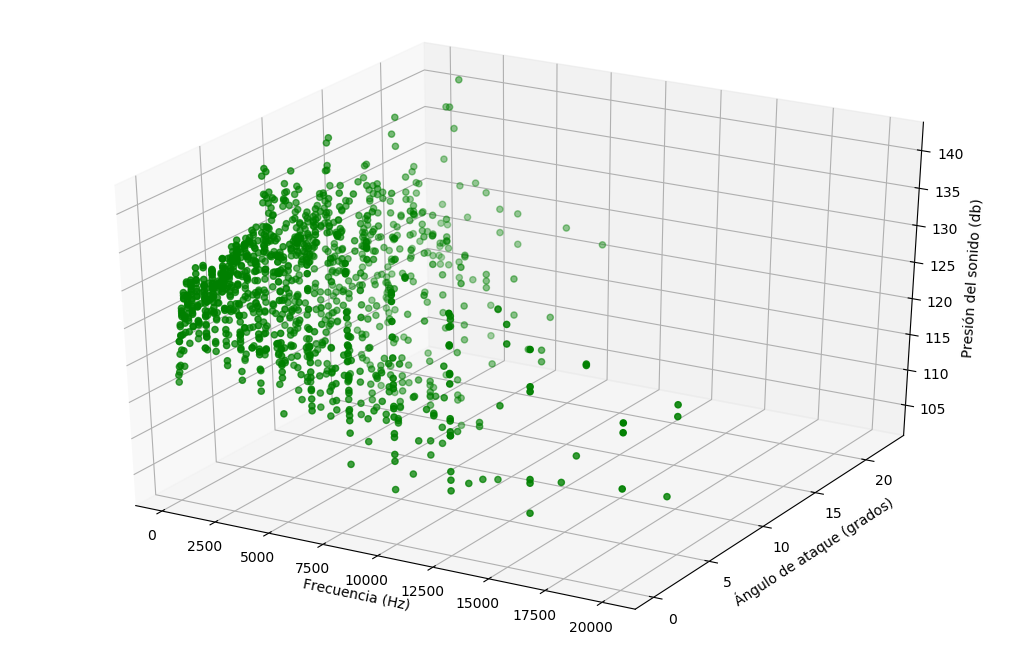
\includegraphics[scale=.6]{Figure_1}
  \caption{Frecuencia Vs. Ángulo de ataque}
  \label{fig:Figure_1}
  \end{center}
\end{figure}

\begin{figure}[H]
  \begin{center}
  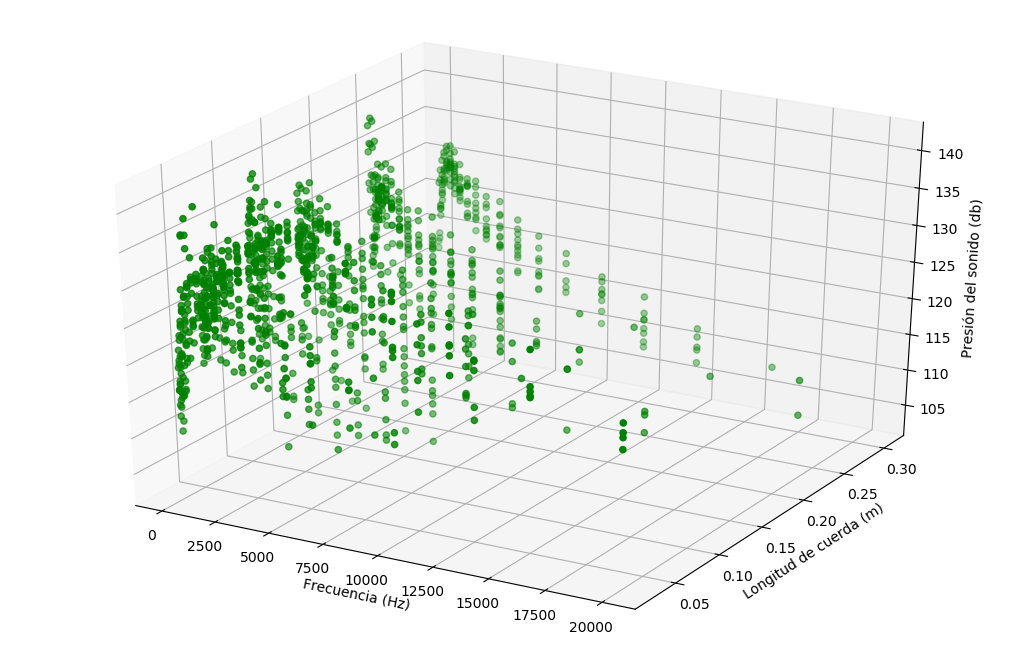
\includegraphics[scale=.6]{Figure_2}
  \caption{Frecuencia Vs. Longitud de cuerda}
  \label{fig:Figure_2}
  \end{center}
\end{figure}

\begin{figure}[H]
  \begin{center}
  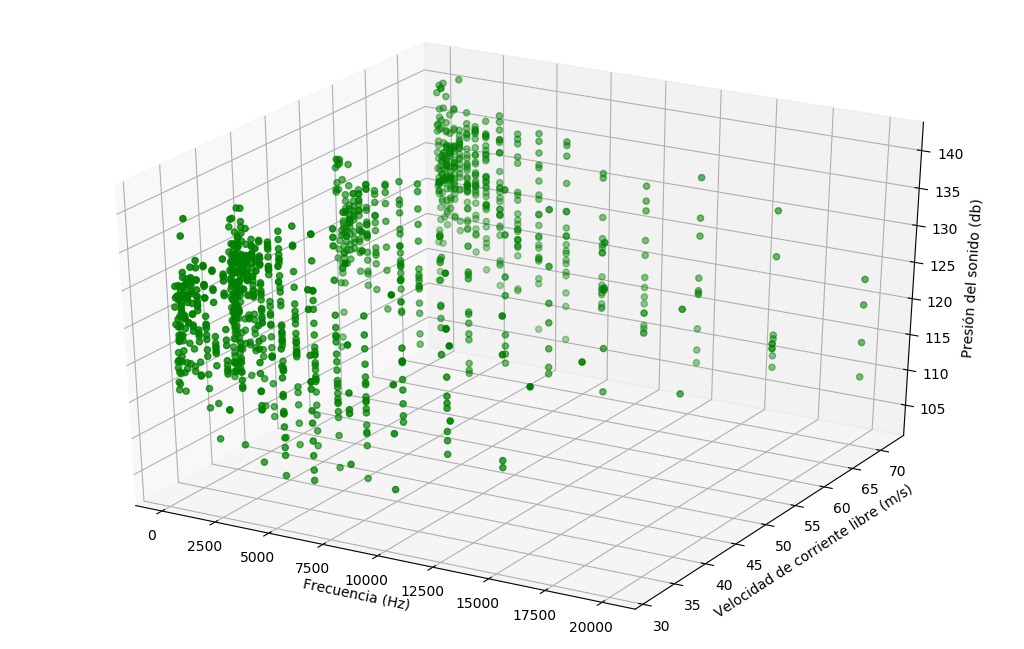
\includegraphics[scale=.6]{Figure_3}
  \caption{Frecuencia Vs. Velocidad de corriente libre}
  \label{fig:Figure_3}
  \end{center}
\end{figure}

\begin{figure}[H]
  \begin{center}
  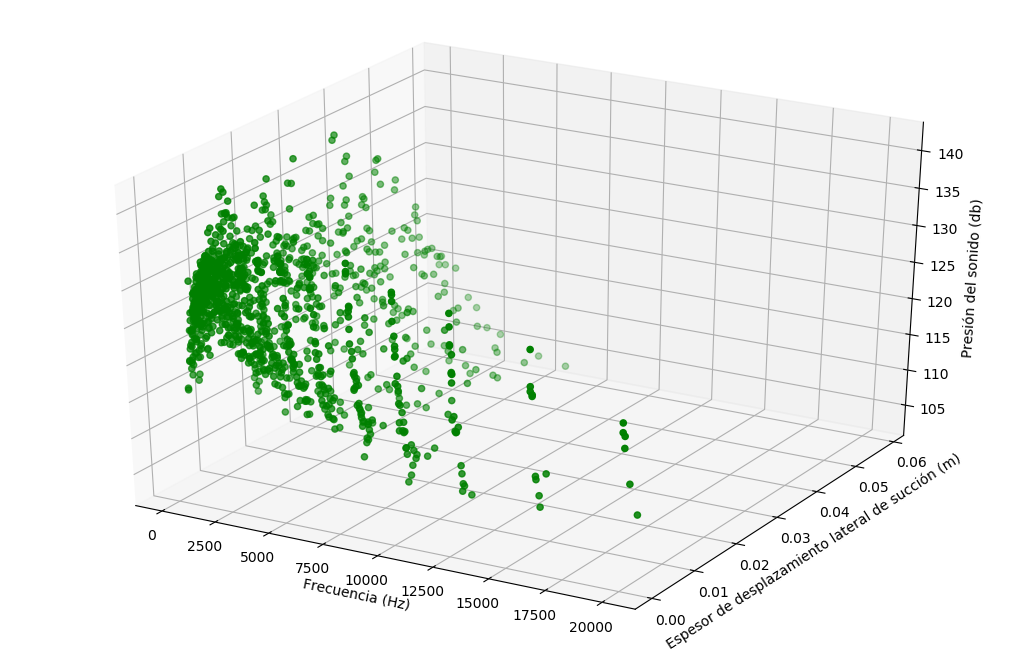
\includegraphics[scale=.6]{Figure_4}
  \caption{Frecuencia Vs. Espesor de desplazamiento lateral de succión}
  \label{fig:Figure_4}
  \end{center}
\end{figure}

\begin{figure}[H]
  \begin{center}
  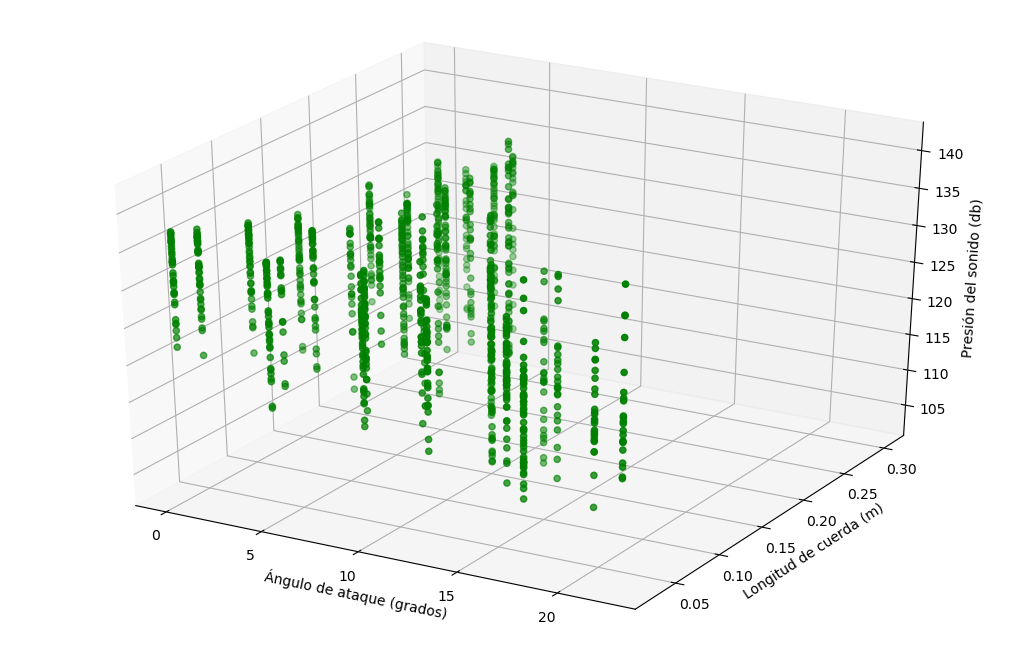
\includegraphics[scale=.6]{Figure_5}
  \caption{Ángulo de ataque Vs. Longitud de cuerda}
  \label{fig:Figure_5}
  \end{center}
\end{figure}

\begin{figure}[H]
  \begin{center}
  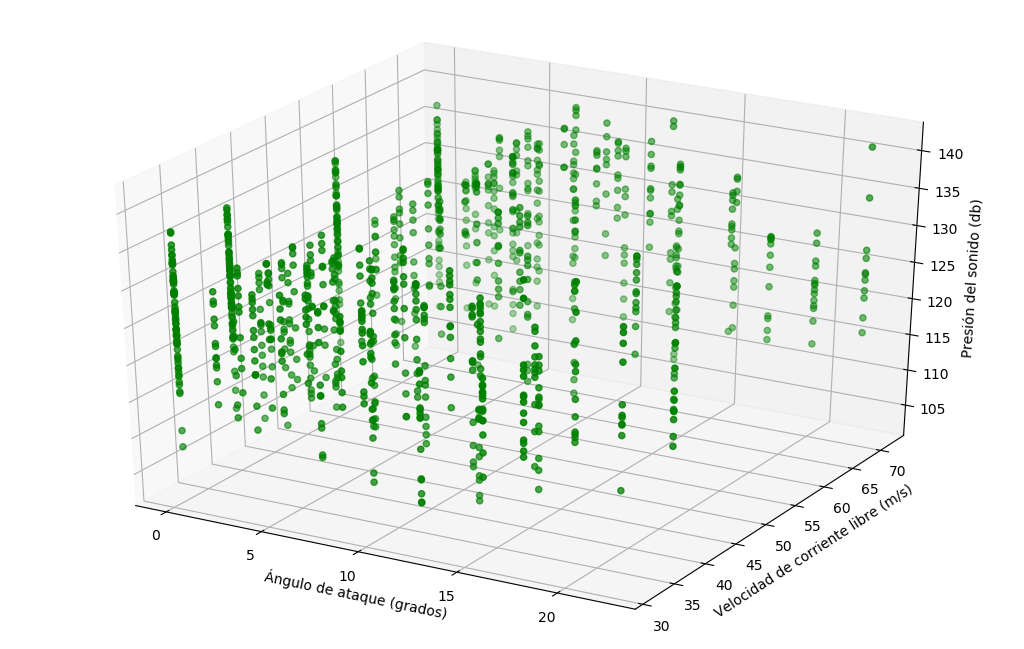
\includegraphics[scale=.6]{Figure_6}
  \caption{Ángulo de ataque Vs. Velocidad de corriente libre}
  \label{fig:Figure_6}
  \end{center}
\end{figure}

\begin{figure}[H]
  \begin{center}
  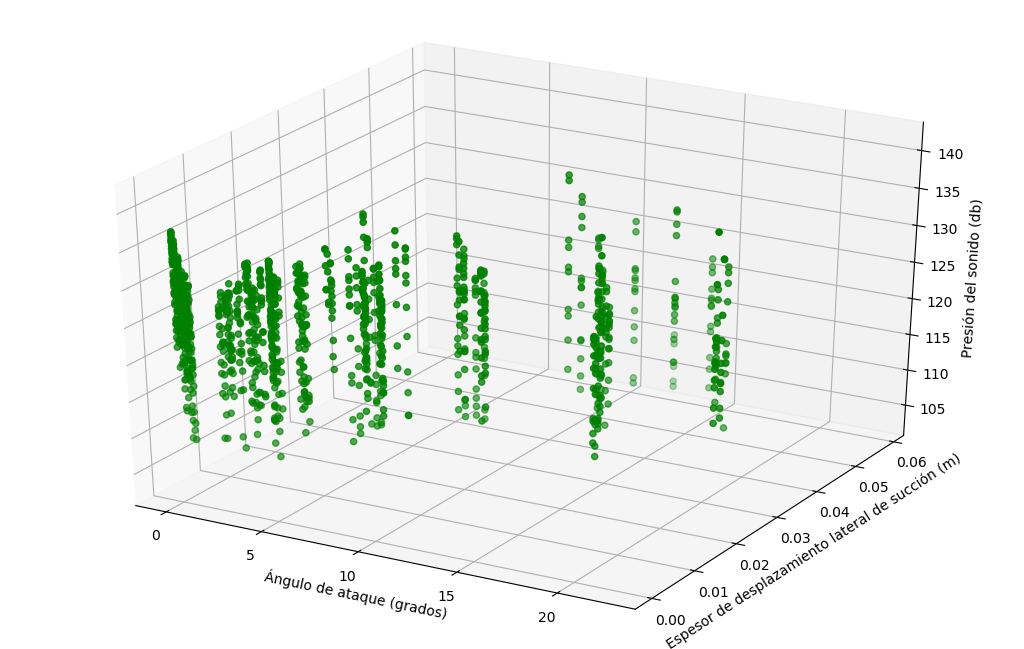
\includegraphics[scale=.6]{Figure_7}
  \caption{Ángulo de ataque Vs. Espesor de desplazamiento lateral de succión}
  \label{fig:Figure_7}
  \end{center}
\end{figure}

\begin{figure}[H]
  \begin{center}
  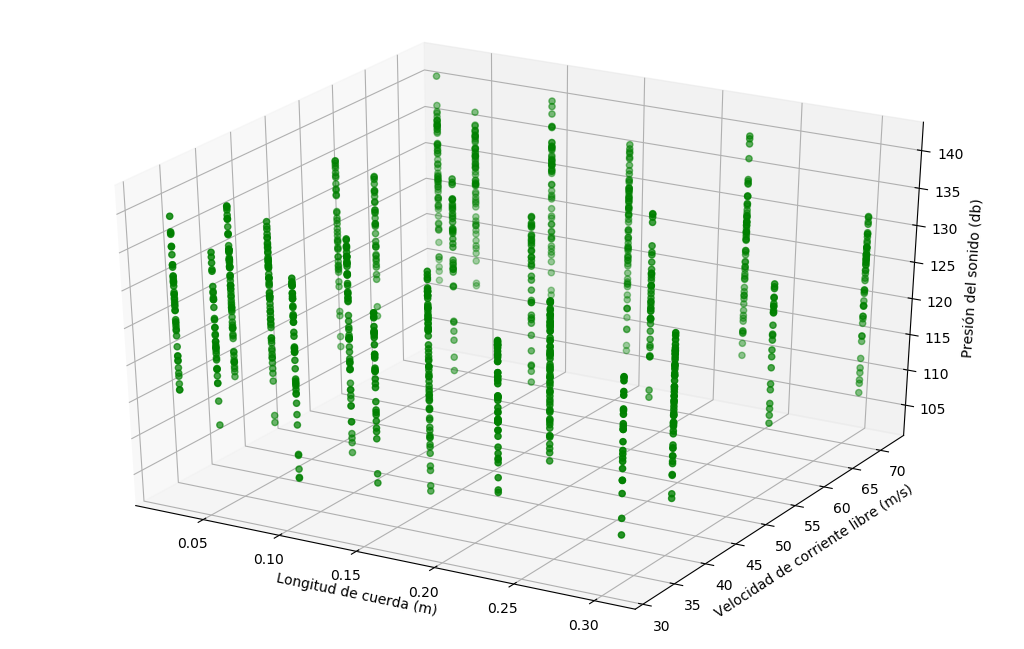
\includegraphics[scale=.6]{Figure_8}
  \caption{Longitud de Cuerda Vs. Velocidad de corriente libre}
  \label{fig:Figure_8}
  \end{center}
\end{figure}

\begin{figure}[H]
  \begin{center}
  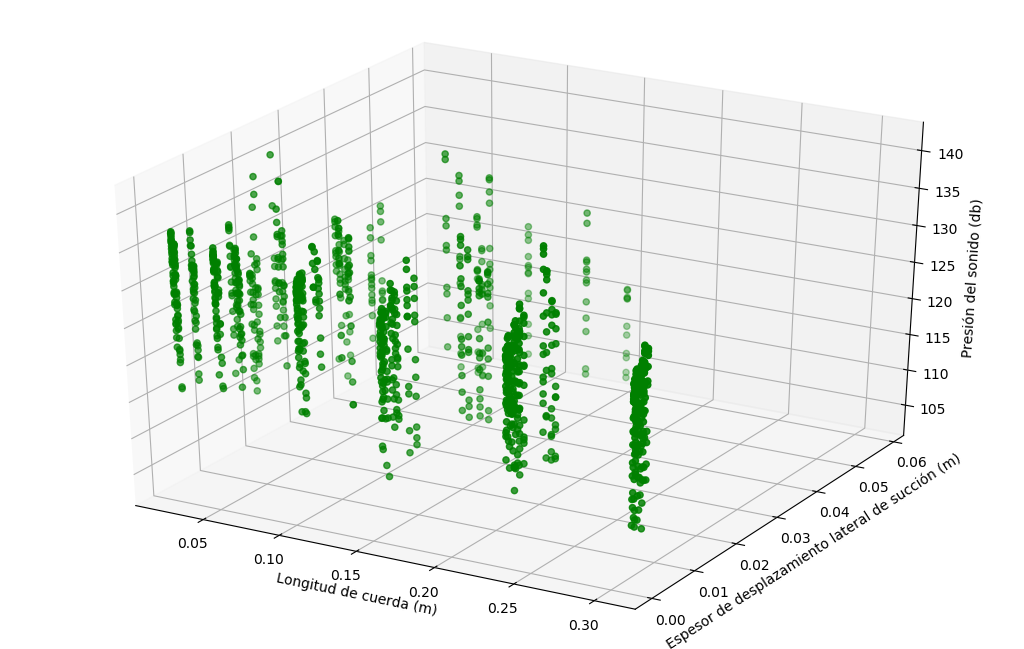
\includegraphics[scale=.6]{Figure_9}
  \caption{Longitud de cuerda Vs. Espesor de desplazamiento lateral de succión}
  \label{fig:Figure_9}
  \end{center}
\end{figure}

\begin{figure}[H]
  \begin{center}
  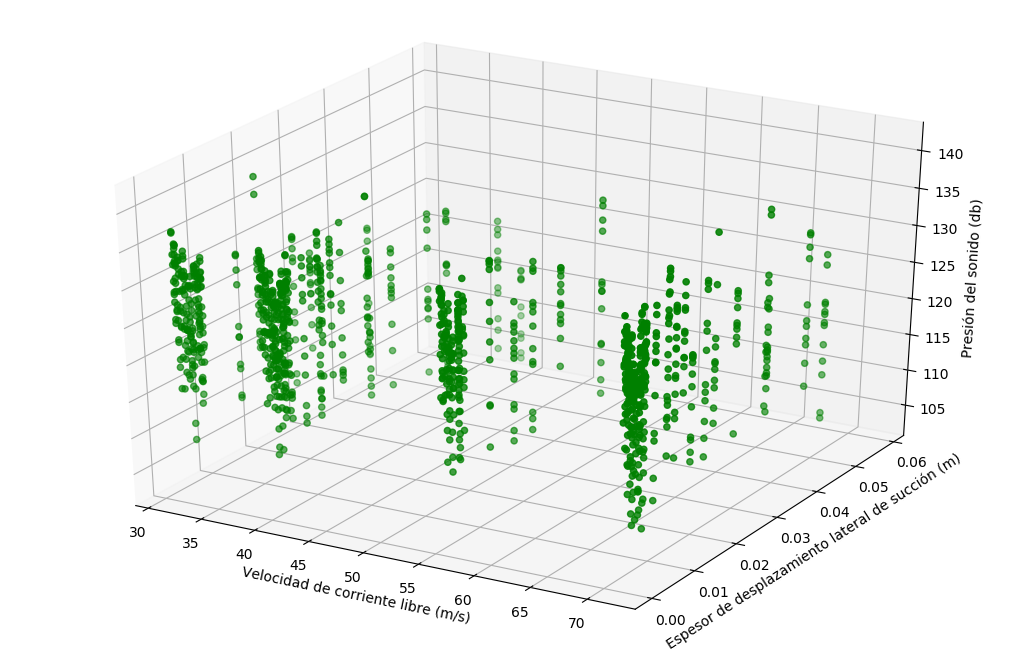
\includegraphics[scale=.6]{Figure_10}
  \caption{Velocidad de corriente libre Vs. Espesor de desplazamiento lateral de succión}
  \label{fig:Figure_10}
  \end{center}
\end{figure}

Se pueden apreciar algunas distribuciones y tendencias a formar ciertos cúmulos, como es el caso de la figura \ref{fig:Figure_4} (Frecuencia Vs. Espesor de desplazamiento lateral de succión), pero los datos no son fáciles de interpretar. En algunas de las características los valores usados no se distribuyen a lo largo de un intervalo, si no que son pocos valores de un pequeño conjunto que se repiten, como es el caso de la ``Velocidad de corriente libre''.

Graficamos únicamente la salida: en el eje X cada elemento y en el eje Y su salida.

\begin{figure}[H]
  \begin{center}
  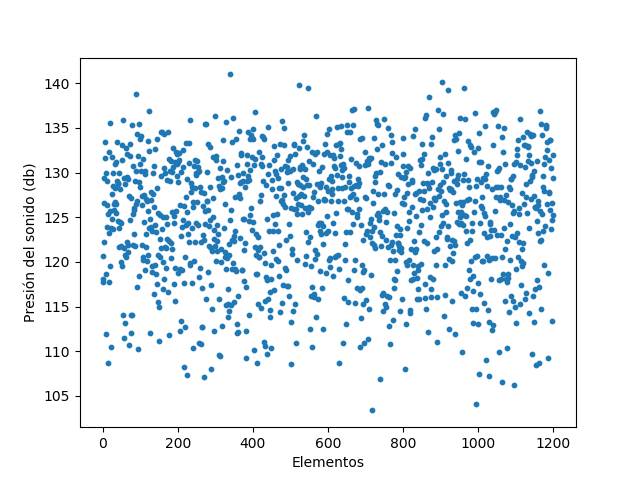
\includegraphics[scale=0.9]{s1}
  \caption{Salida de datos de training.}
  \label{fig:s1}
  \end{center}
\end{figure}

Parece ser una distribución uniforme sin tendencias ni patrones. Para detectar tendencias, ordenamos las salidas de menor a mayor.

\begin{figure}[H]
  \begin{center}
  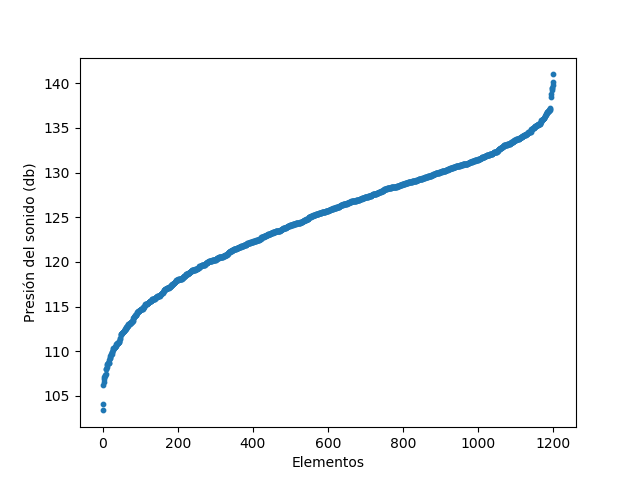
\includegraphics[scale=0.9]{s2}
  \caption{Salida de datos de training, ordenados de menor a mayor.}
  \label{fig:s2}
  \end{center}
\end{figure}

Se puede apreciar claramente que la salida sigue una función ``logit''; no podemos esperar los mejores resultados si ajustamos con un modelo lineal a no ser que se haga una transformación. Debido a la dificultad de ello (y la falta de entendimiento del problema como se comentó con anterioridad), no se hará.

\subsection{Funciones a usar}

Dado que debemos predecir un valor continuo, se utilizará Regresión Lineal. Aprovechamos el trabajo realizado en la primera práctica y utilizamos SGD: el algoritmo hallará los pesos o coeficientes $W$ de una función lineal que predecirá la salida, donde la función de coste es MSE; buscamos minimizar lo mayor posible la distancia entre nuestra predicción y la salida verdadera. Utilizamos un tamaño de \textit{minibatch} bajo, 4, para acelerar los cálculos, y utilizamos un \textit{learning rate} de 0.01, igual que en prácticas anteriores debido a sus buenos resultados. Se ejecutará el algoritmo miles de iteraciones (10.000) para conseguir convergencia y obtener un ajuste lo más cercano posible. No se aplicará regularización: sabemos de hecho que el ajuste lineal no será el mejor para este tipo de problema, por lo que aplicar regularización no ayudará mucho.

Antes de ejecutar SGD, se debe añadir a cada tupla del conjunto el valor 1.0, para el coeficiente independiente de $W$.

\subsection{Entrenamiento y test}

Se ha ejecutado SGD con el junto de training, y se han obtenido los siguientes pesos:

$W = [ 0.8345524  -0.63795127 -0.27559551 -0.26757449  0.10771084 -0.1976129 ]$

Posteriormente se obtuvieron las predicciones con el conjunto de salida.

Los errores han sido:

$E_{in} = 0.01616$

$E_{out} = 0.01868$

\subsection{Conclusiones}

Los errores son bajos y casi similares, por lo que se puede considerar como un buen ajuste. El error de salida es ligeramente superior al de entrada, por lo que podemos asumir que se ha producido algo de sobreajuste. Puede ser debido a que no se ha utilizado \textit{Cross-validation}, y el conjunto de entrenamiento fue mayor al de salida.

Graficamos los resultados, dado que no se esperaba un ajuste decente al ser la salida una sigmoide. En las figuras \ref{fig:s3} y \ref{fig:s4} se ven, normalizadas, las salidas de los conjuntos de entrada y salida con sus predicciones.

Aunque los puntos siguen la tendencia de la sigmoide, se puede ver claramente una gran dispersión existente entre las predicciones (naranja) y las salidas verdaderas (azul). Como se comentó con anterioridad, un modelo lineal no parece ser el mejor para este tipo de problema, donde la salida claramente no es lineal y las entradas siguen tendencias difíciles de interpretar. La gran dispresión de las predicciones respecto a la salida es prueba de ello.

Aún así, se han conseguido errores bastante bajos y similares: el entrenamiento permite realizar predicciones con el mismo nivel de error.

\begin{figure}[H]
  \begin{center}
  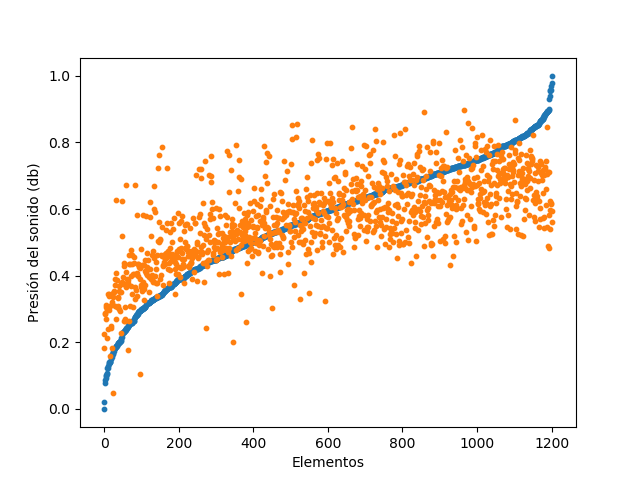
\includegraphics[scale=0.8]{s3}
  \caption{Salida de datos de training (azul) junto con las predicciones (naranja) para ajuste con SGD.}
  \label{fig:s3}
  \end{center}
\end{figure}

\begin{figure}[H]
  \begin{center}
  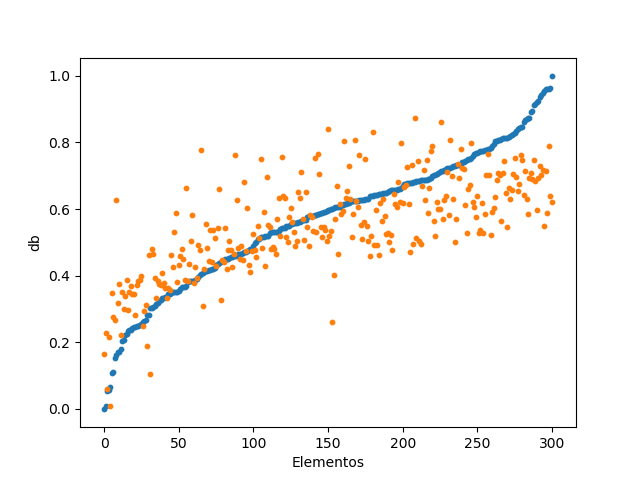
\includegraphics[scale=0.8]{s4}
  \caption{Salida de datos de test (azul) junto con las predicciones (naranja) para ajuste con SGD.}
  \label{fig:s4}
  \end{center}
\end{figure}


\subsection{EXTRA: Ajuste no lineal}

Se ha decidido probar un ajuste no lineal para compararlo con el lineal. Se ha utilizado Random Forest, ejecutándose con los parámetros por defecto de SKLearn pero con un mayor número de árboles, 100.

En las figuras \ref{fig:s5} y \ref{fig:s6} se ven los resultados.

Se puede ver un mejor ajuste que en el caso lineal, como era de esperar.

Los errores han sido:

$E_{in} = 0.00031$

$E_{out} = 0.00489$

El error de entrada ha sido mucho menor que el de entrada; en las figuras se puede ver claramente que se ha producido \textit{overfitting}. Aún así, el error de salida es mucho menor que en el modelo lineal.

\begin{figure}[H]
  \begin{center}
  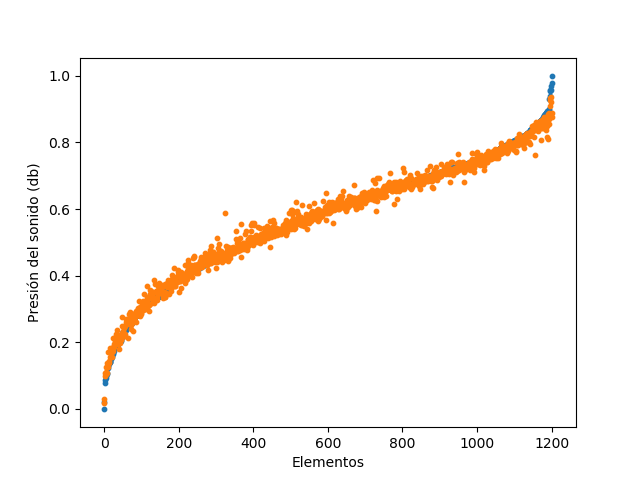
\includegraphics[scale=0.8]{s5}
  \caption{Salida de datos de training (azul) junto con las predicciones (naranja) para ajuste con Random Forest.}
  \label{fig:s5}
  \end{center}
\end{figure}

\begin{figure}[H]
  \begin{center}
  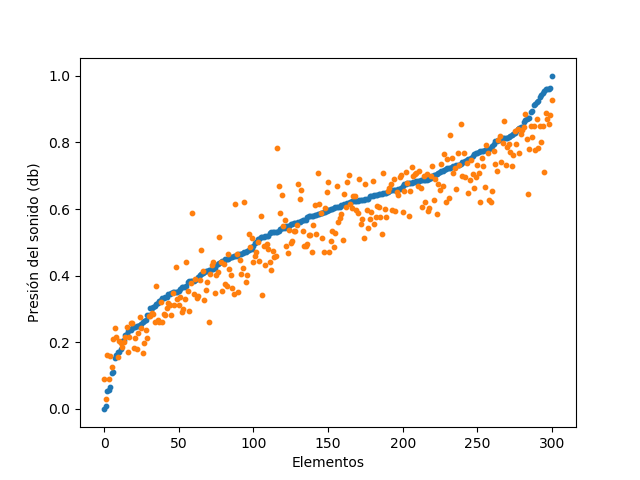
\includegraphics[scale=0.8]{s6}
  \caption{Salida de datos de test (azul) junto con las predicciones (naranja) para ajuste con Random Forest.}
  \label{fig:s6}
  \end{center}
\end{figure}

%----------------------------------------------------------------------------------------
%	BIBLIOGRAFIA
%----------------------------------------------------------------------------------------
\newpage

\section{Bibliografía}

\noindent
Vladimir Cherkassky, Filip Mulier
\\
\textit{LEARNING FROM DATA: Concepts, Theory, and Methods}.
\\
\\
\\
Se ha utilizado como bibliografia adicional PDFs ofrecidos por el profesorado y el guión de prácticas.

%----------------------------------------------------------------------------------------
%	FIN DEL DOCUMENTO
%----------------------------------------------------------------------------------------

\end{document}